
\subsection{Führungsschaufel}


\begin{zebratabular}{p{4.5cm}p{\textwidth-5.3cm}}
	\rule{0pt}{11pt}\textit{Tester}           & Pascal Roth und Matteo Trachsel \\ 
	\rule{0pt}{11pt}\textit{Datum}:           & 13.03.2015\\
	\rule{0pt}{11pt}\textit{Beschreibung}:    & Das Ziel des Testes besteht darin, verschieden Führungsschaufeln zu testen und eine geeignete Befestigung zu finden.\\
	\rule{0pt}{11pt}\textit{Akteure}:         & Riemen und Führunsschaufeln\\
	\rule{0pt}{11pt}\textit{Bedingung}:       & Für den Test wurden aus einem 1 mm dicken Aluminiumblech, welches bereits auf die Breite des Förderbandes zugeschnitten wurde, verschieden Lange Stücke abgeschnitten. Da pro Tennisball zwei Führungsschaufeln vorne und hinten benötigt werden, gibt es zwei Möglichkeiten zur Gestaltung der Führungsschaufeln. Die erste Möglichkeit besteht darin, dass immer eine einzelne Schaufel für je vorne und hinten realisiert wird. Die zweite Möglichkeit besteht darin, dass man die hinter und die nächste vorne liegende Führungschaufel zusammen in einem Blechstück realisiert.\\
	\rule{0pt}{11pt}\textit{Erwartete Fehlermeldung}:          & keine \\
	\rule{0pt}{11pt}\textit{Vorgehen}:        & Riemen manuell auf den Achsen antreiben, Drehmoment für die Welle festlegen, optimale Führungsschaufel herstellen \\
	\rule{0pt}{11pt}\textit{Erwartetes Ergebnis}: & Durch den Versuch stellte sich heraus, dass es sich besser eignet, wenn zwei Führungsschaufeln zusammen in einem Blechstück realisiert werden. Wenn die Führungschaufelpaare mit dem UHU Kleber am vorderen Rand angeklebt werden, können sie immer noch den Radius der Wellen überfahren, ohne sich abzulösen. Zur Sicherheit können die Führungsschaufeln noch mit einem Klebeband befestigt werden. \\
	\rule{0pt}{11pt}\textit{Eingetretenes Ergebnis}: & Alles IO.\\
	\rule{0pt}{11pt}\textit{Test bestanden?}:     & Ja \\
\end{zebratabular}  



\begin{figure}[h!]
	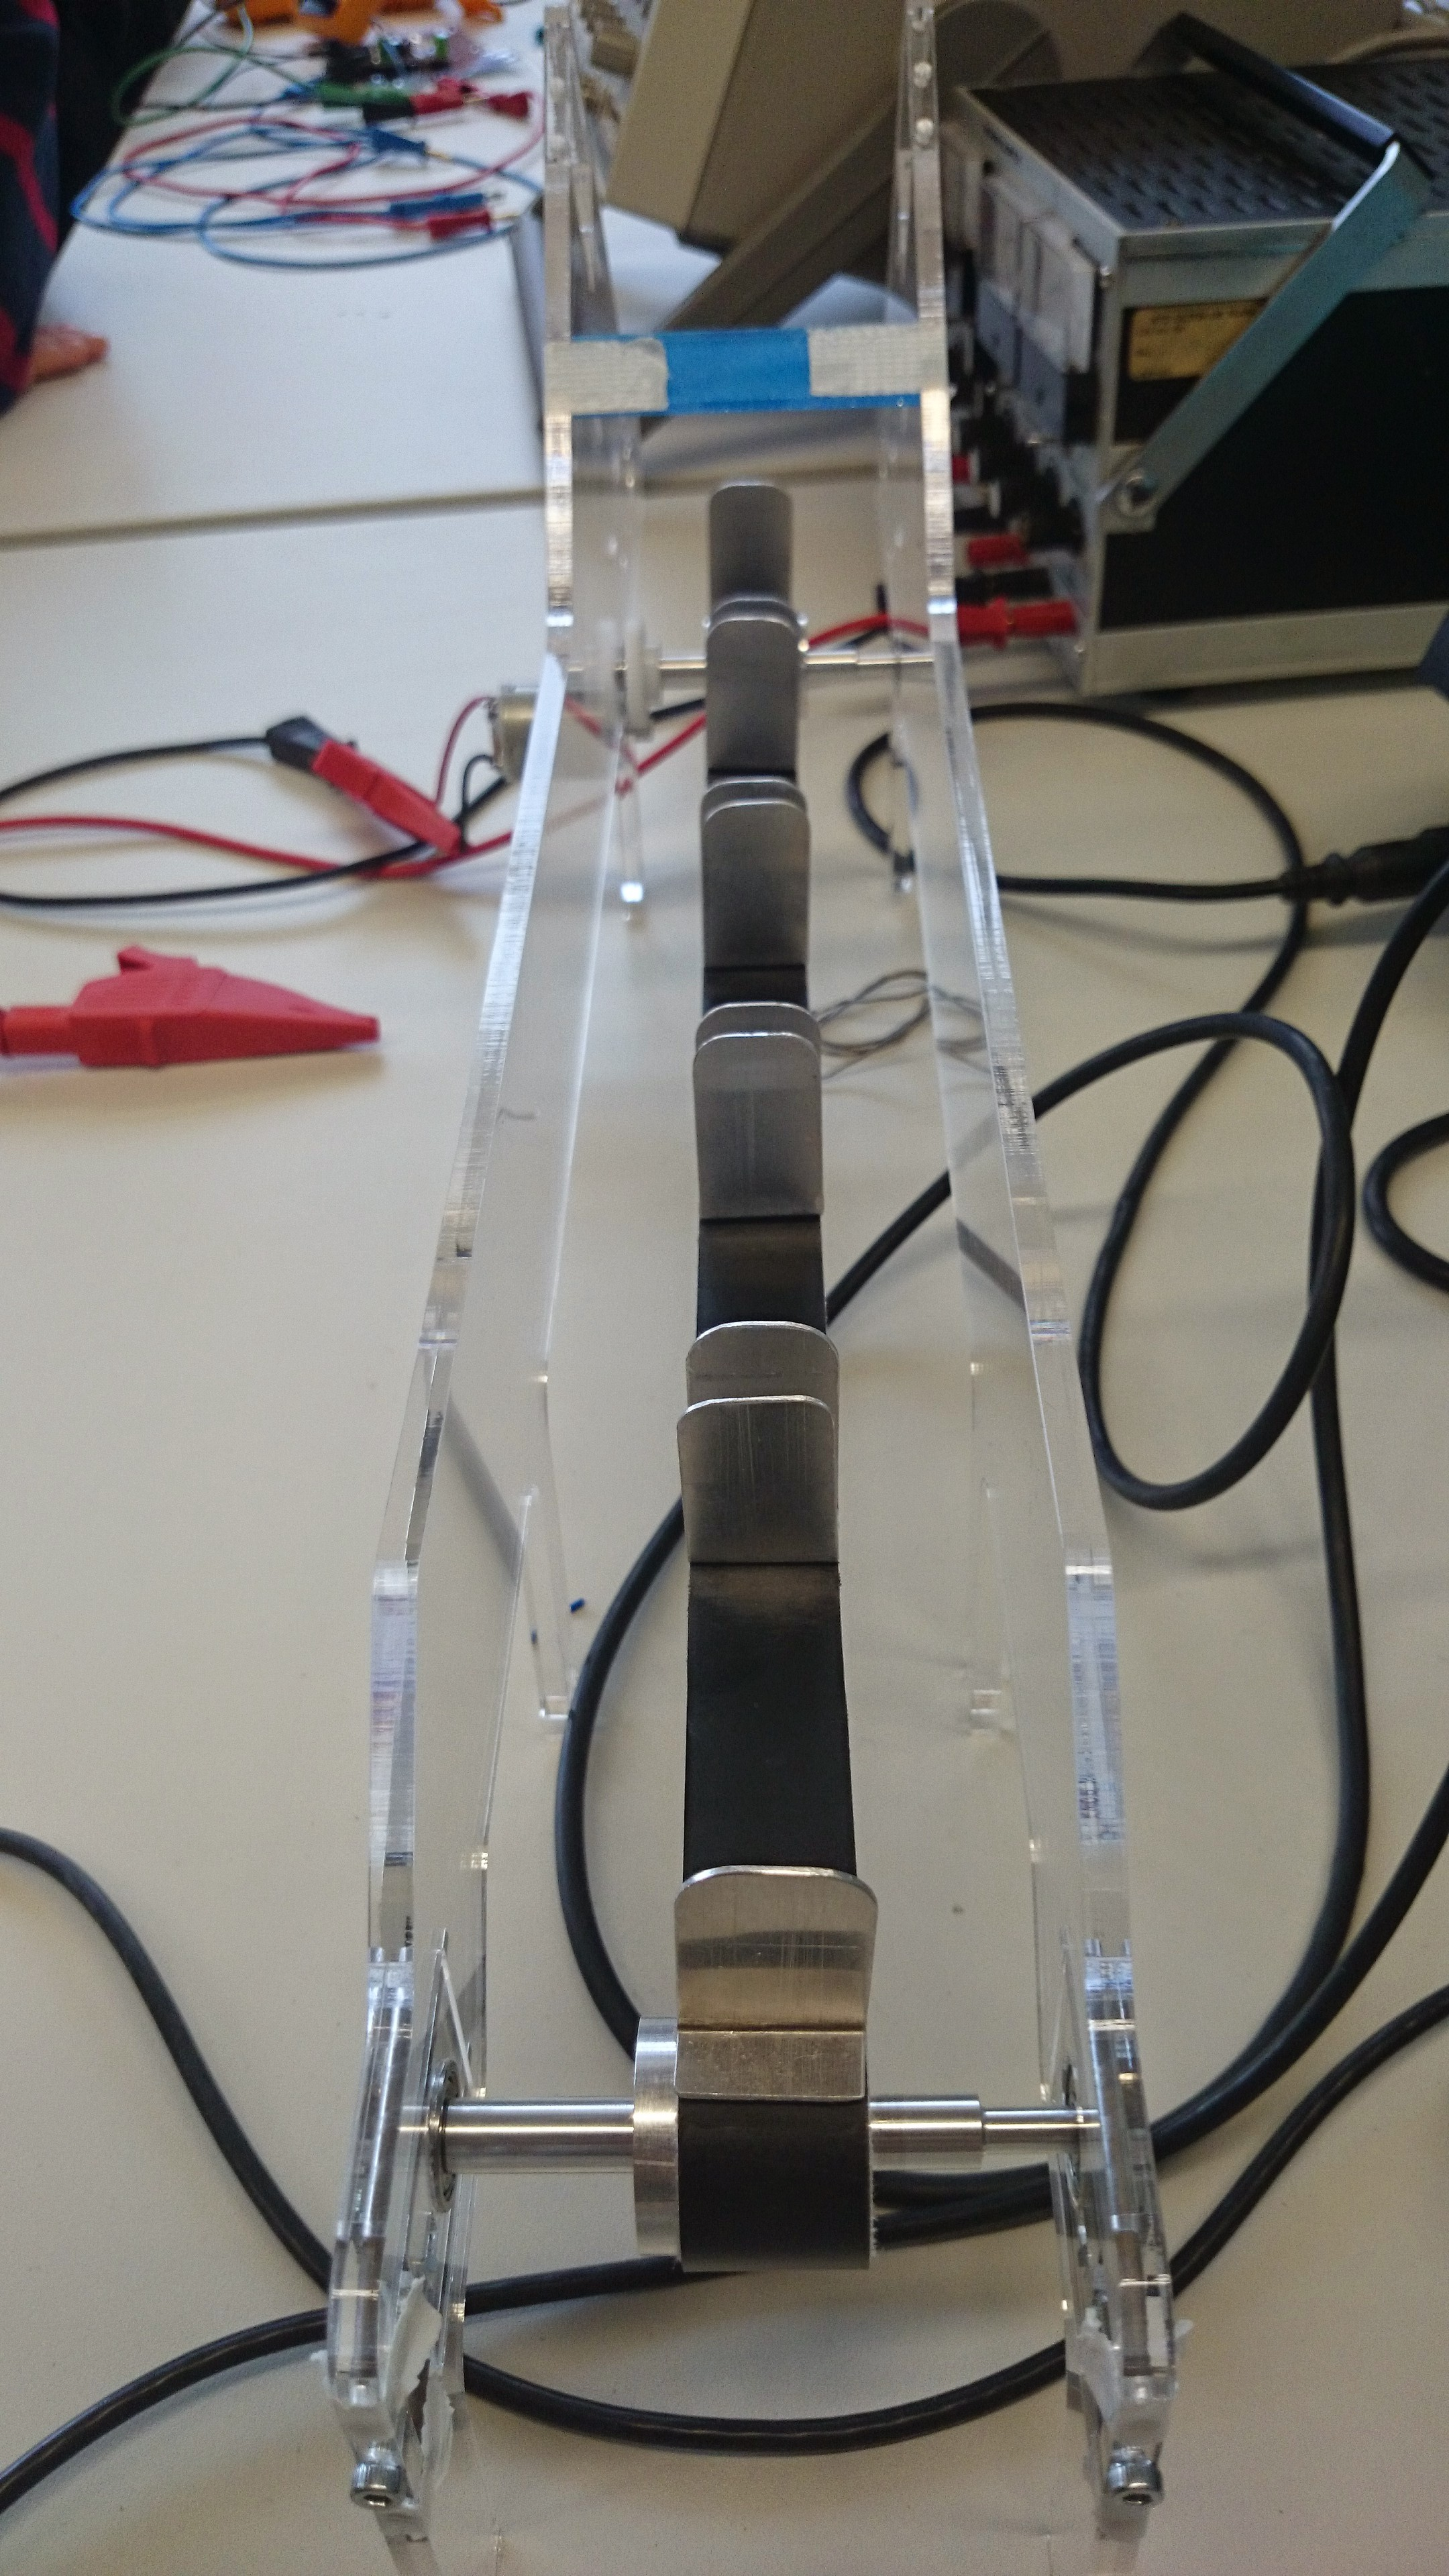
\includegraphics[width=0.3\textwidth,clip,trim=0cm 0cm 0cm 0cm]
	{Testberichte/Fuehrungsschaufel.jpg}
	\centering
	\caption{Förderband mit Führungschaufeln}
	\label{abb:Führungsschaufel}
\end{figure}


